 
\section*{Aufgabe 1: \emph{Maxwell'sche Geschwindigkeitsverteilung}}

\begin{equation}
f(v)=N\left(\frac{m}{2\pi k_BT}\right)^\frac{3}{2}\exp{\left(-\frac{mv²}{2k_bT}\right)}\cdot4\pi v²
\end{equation}

Die Normalisierungkonstante berechnet sich mit Hilfe von

\begin{equation}
\int_{-\infty}^\infty f(v)\text{d}v=1.
\end{equation}

\begin{itemize}
\item[a)] Die wahrscheinlichste Geschwindigkeit ist gegeben durch
\begin{equation}
\frac{\text{d}f(v)}{\text{d}v}=0.
\end{equation}

\item[b)] Die mittlere Geschwindigkeit ist 

\begin{equation}
\bar{v}=\int_{-\infty}^\infty v\cdot f(v)\text{d}v.
\end{equation}



\item[c)]
\item[d)]
\item[e)]
\end{itemize}

\section*{Aufgabe 2: \emph{Binning}}
\begin{itemize} 
\item[a)] Die Strukutur der Häufigkeitsverteilung wird in einem Histogramm mit niedrigen 
Binning (Bin 5) nicht deutlich. 
In den Histogrammen mit hohem Binning ($30$, $50$) sind an mehreren Stellen einzelne Peaks.
Für die Verteilungsfunktion bei Größe und Gewicht kann man auf eine solche
genaue Betrachtung allerdings verzichten.
Ein Histogramm mit mittlerer Binning Zahl reicht aus um die Verteilungsfunktion abzuleiten und ist übersichtlich, also ist das Binning mit $15$ Bins sinnvoll.

\item[b)] Verwendet man weit mehr Daten als die vorgegeben 250, so sollte sich nicht grundlegend die
Struktur der abgebildeten Verteilungsfunktion ändern.
Die Bin-Breite sollte zumindest so gewählt werden, dass mehrere Punkte gruppiert werden. Als minimale Bin-Breite kann also für Gewicht 1 - 5 kg gewählt werden, da die Datensätze auf \SI{0.01}{\kilogram} genau angegeben sind.\\
Bei der Größenverteilung sind die Daten
auf \SI{0.01}{\metre} genau angegeben, daher ist eine sinnvolle minimale Bin-Breite \SI{0.05}{\metre}. 
%Der Höchstwert der Gewichtsverteilung ist das 100-fache der minimalen Differenz zweier Werte. Bei der Größenverteilung das 5-fache. Allerdings hat die Groessenverteilung lediglich ein Spektrum von 50 moeglichen Werten (1.50 - 2.00), die Gewichtsverteilung dagegen wesentlich mehr.	

\item[c)]
Die Histogramme zeigen mit steigenem Binning (5, 10, 15, 20) deutlich,
dass die relative Höhendifferenz zweier Bins mit steigenden Werten ebenfalls zunimmt (exponentiell).
Bei den hohen Binnings (30, 50) wird dieser gleichbleibende Trend jedoch von einzelnen Bins unterbrochen.

\begin{figure}
\centering
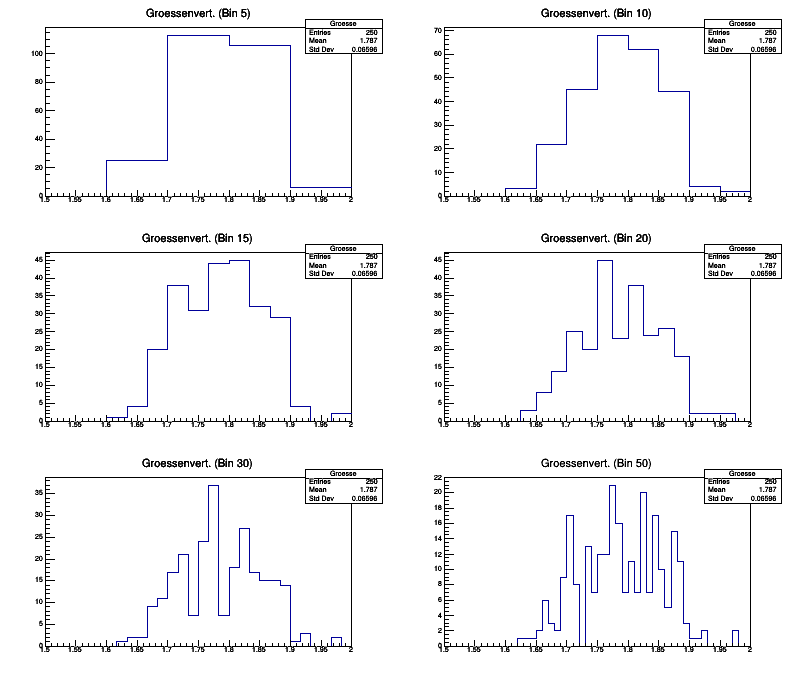
\includegraphics[width=\textwidth]{GroessenverteilungBinnings2x3.png}
\caption{Histogramme der Größenverteilung mit verschiedenen Binnings.}
\end{figure}

\begin{figure}
\centering
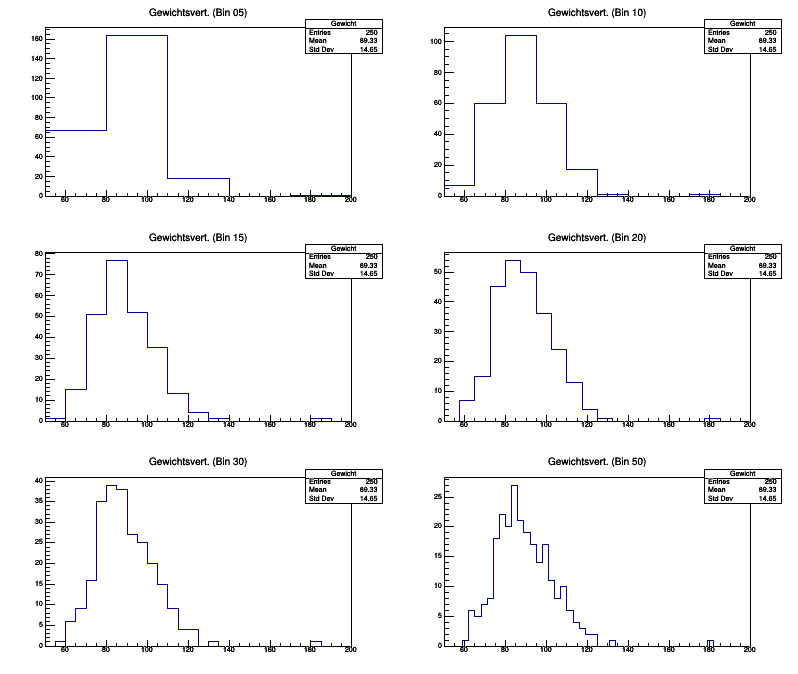
\includegraphics[width=\textwidth]{GewichtsverteilungBinnings2x3.png}
\caption{Histogramme der Gewichtsverteilung mit verschiedenen Binnings.}
\end{figure}

\begin{figure}
\centering
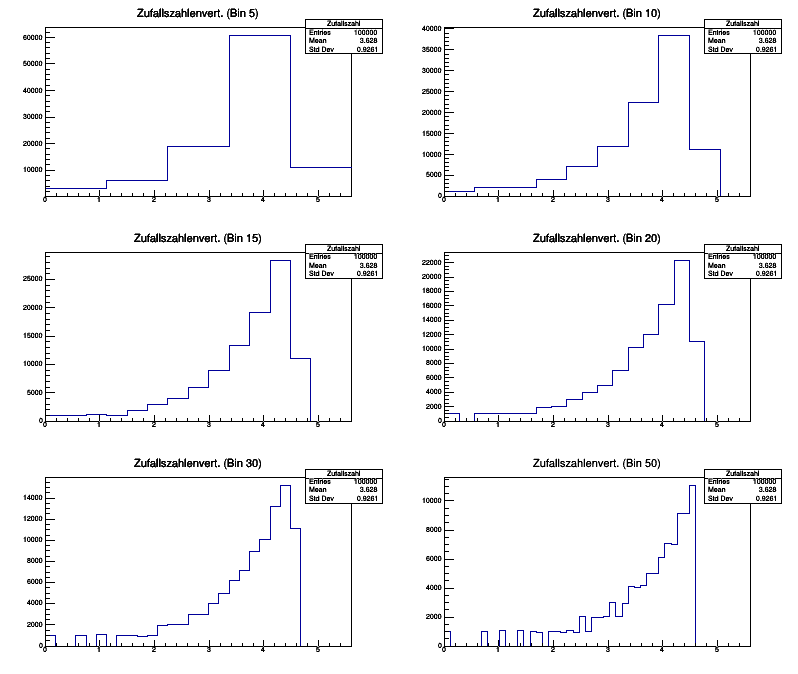
\includegraphics[width=\textwidth]{Log_ZufallszahlenverteilungBinnings2x3.png}
\caption{Logarithmierte Zufallszahlen zwischen $1$ und $100$ mit verschiedenen Binnings.}
\end{figure}

\end{itemize}
\section*{Aufgabe 3: \emph{Würfel}}
\begin{itemize}
\item[a)] Die Summe der Punkte ergibt $9$. 
\begin{align*}
P(W_{\text{r}} + W_{\text{b}} = 9) \\
 = 2P(9|W_{\text{r,b}} = 3 ) \\
 + 2P(9|W_{\text{r,b}} = 4 ) \\
 + 2P(9|W_{\text{r,b}} = 5 ) \\
 + 2P(9|W_{\text{r,b}} = 6 ) \\
 = 2/36 + 2/36 + 2/36 + 2/36 \\
 = 1/6
\end{align*}

\item[b)] Die Summe der Punkte ist $9$ oder mehr.
\begin{align*}
P(W_{\text{r}} + W_{\text{b}} > 9) \\
 = 2P(9|W_{\text{r,b}} = 4 ) \\
 + 2P(9|W_{\text{r,b}} = 5 ) \\
 + 2P(9|W_{\text{r,b}} = 6 ) \\
 = 2 \cdot 1/6 \cdot 1/6 + 2 \cdot 1/6 \cdot 1/3 + 2 \cdot 1/6 \cdot 1/2 \\
 = 1/3
\end{align*}

\item[c)] Die Wahrscheinlichkeit, dass ein Würfel $4$, der andere $5$ Punkte zeigt.
\begin{align*}
P(W_{\text{r,b}} = 5 \land W_{\text{r,b}}=4)\\
= 2P(W_{\text{r,b}} = 5) + 2P(W_{\text{r,b}} = 4)\\
= 2/3
\end{align*}

\item[d)] Die Wahrscheinlichkeit, dass der rote Würfel $4$ und 
der blaue $5$ Punkte zeigt.

\begin{align*}
P(W_{\text{r}} = 4 \land W_{\text{b}}=5)\\
= 1/3
\end{align*}

\item[e)] Die Summe der Punkte ist $9$ unter der Bedingung, dass der rote Würfel eine $4$ zeigt.
\begin{align*}
P(W_{\text{r}} + W_{\text{b}} = 9|W_{\text{r}} = 4)
= 1/6
\end{align*}


\item[f)] Die Summe der Punkte ist $9$ oder mehr unter der Bedingung, dass der rote Würfel eine $4$ zeigt.
\begin{align*}
P(W_{\text{r}} + W_{\text{b}} > 9|W_{\text{r}} = 4)
= P(W_{\text{b}} = 6|W_{\text{r}} = 4) + P(W_{\text{b}} = 5|W_{\text{r}} = 4)\\
= 1/6 + 1/6 = 2/3 
\end{align*}


\item[g)]Die Wahrscheinlichkeit, dass der rote Würfel $4$ und der blaue $5$ Punkte zeigt.
\begin{align*}
P(W_{\text{r}} = 4|W_{\text{r}} = 4) + P(W_{\text{b}} = 5|W_{\text{r}} = 4)\\
=1/6
\end{align*}
\end{itemize}

\section*{Aufgabe 4: \emph{Zweidimensionale Gaußverteilung}}

\begin{itemize}
\item[a)] Der Korellationskoeffizient berechnet sich mit
\begin{equation}
\rho(x,y)=\frac{\text{Cov}(x,y)}{\sigma_x\cdot\sigma_y}
\end{equation}
zu $\rho(x,y)=0.8.$

\item[b)] Helena schreibt auf. Siehe Vorlesung.


\end{itemize}
